\documentclass[11pt]{article}
\usepackage[utf8]{inputenc}
\usepackage{geometry}
\usepackage{url}
\usepackage{hyperref}
\usepackage{epsfig}
\usepackage{graphicx}
\usepackage[most]{tcolorbox}
\usepackage[export]{adjustbox}
\geometry{a4paper}
\geometry{margin=1in}

\usepackage[sorting=none, backend=bibtex]{biblatex}
\usepackage{filecontents}
\usepackage{tabularx}

\def\etal{\emph{et al}.\ }
\newcommand{\CPP}
{C\nolinebreak[4]\hspace{-.05em}\raisebox{.22ex}{\footnotesize\bf ++\ }}

\begin{filecontents}{final-report-references.bib}

@article{lau2016empirical,
  title={An Empirical Evaluation of doc2vec with Practical Insights into Document Embedding Generation},
  author={Lau, Jey Han and Baldwin, Timothy},
  journal={arXiv preprint arXiv:1607.05368},
  year={2016}
}

@inproceedings{mikolov2013distributed,
  title={Distributed representations of words and phrases and their compositionality},
  author={Mikolov, Tomas and Sutskever, Ilya and Chen, Kai and Corrado, Greg S and Dean, Jeff},
  booktitle={Advances in neural information processing systems},
  pages={3111--3119},
  year={2013}
}

@article{mikolov2013efficient,
  title={Efficient estimation of word representations in vector space},
  author={Mikolov, Tomas and Chen, Kai and Corrado, Greg and Dean, Jeffrey},
  journal={arXiv preprint arXiv:1301.3781},
  year={2013}
}

@inproceedings{le2014distributed,
  title={Distributed Representations of Sentences and Documents.},
  author={Le, Quoc V and Mikolov, Tomas},
  booktitle={ICML},
  volume={14},
  pages={1188--1196},
  year={2014}
}

@misc{wikidatadump2016,
  author="Meta",
  title="Data dump torrents --- Meta{,} discussion about Wikimedia projects",
  year="2016",
  url={https://meta.wikimedia.org/w/index.php?title=Data_dump_torrents},
  note="[Online; accessed 9-August-2016]"
}

@inproceedings{broder1997resemblance,
  title={On the resemblance and containment of documents},
  author={Broder, Andrei Z},
  booktitle={Compression and Complexity of Sequences 1997. Proceedings},
  pages={21--29},
  year={1997},
  organization={IEEE}
}

@misc{keras,
  title={Keras: Deep Learning library for Theano and TensorFlow},
  url={https://keras.io/}
}

@inproceedings{gensim,
  title = {{Software Framework for Topic Modelling with Large Corpora}},
  author = {Radim {\v R}eh{\r u}{\v r}ek and Petr Sojka},
  booktitle = {{Proceedings of the LREC 2010 Workshop on New
       Challenges for NLP Frameworks}},
  pages = {45--50},
  year = 2010,
  month = May,
  day = 22,
  publisher = {ELRA},
  address = {Valletta, Malta},
  note={\url{http://is.muni.cz/publication/884893/en}},
  language={English}
}

@misc{chromium2016,
  title={Git repositories on chromium},
  url={https://chromium.googlesource.com/},
  journal={chromium Git repositories}
}

@article{dai2015document,
  title={Document embedding with paragraph vectors},
  author={Dai, Andrew M and Olah, Christopher and Le, Quoc V},
  journal={arXiv preprint arXiv:1507.07998},
  year={2015}
}

@InProceedings{maas2011,
  author    = {Maas, Andrew L.  and  Daly, Raymond E.  and  Pham, Peter T.  and  Huang, Dan  and  Ng, Andrew Y.  and  Potts, Christopher},
  title     = {Learning Word Vectors for Sentiment Analysis},
  booktitle = {Proceedings of the 49th Annual Meeting of the Association for Computational Linguistics: Human Language Technologies},
  month     = {June},
  year      = {2011},
  address   = {Portland, Oregon, USA},
  publisher = {Association for Computational Linguistics},
  pages     = {142--150},
  url       = {http://www.aclweb.org/anthology/P11-1015}
}

@article{maaten2008visualizing,
  title={Visualizing data using t-SNE},
  author={Maaten, Laurens van der and Hinton, Geoffrey},
  journal={Journal of Machine Learning Research},
  volume={9},
  number={Nov},
  pages={2579--2605},
  year={2008}
}

@misc{googlegroups2015,
  title={Google Groups},
  url={https://groups.google.com/d/msg/word2vec-toolkit/q49firnoqro/bp--14e4unwj},
  journal={Google Groups}
}

@article{zhang2010understanding,
  title={Understanding bag-of-words model: a statistical framework},
  author={Zhang, Yin and Jin, Rong and Zhou, Zhi-Hua},
  journal={International Journal of Machine Learning and Cybernetics},
  volume={1},
  number={1-4},
  pages={43--52},
  year={2010},
  publisher={Springer}
}

@article{mesnil2014ensemble,
  title={Ensemble of generative and discriminative techniques for sentiment analysis of movie reviews},
  author={Mesnil, Gr{\'e}goire and Mikolov, Tomas and Ranzato, Marc'Aurelio and Bengio, Yoshua},
  journal={arXiv preprint arXiv:1412.5335},
  year={2014}
}

@article{rumelhart1988learning,
  title={Learning representations by back-propagating errors},
  author={Rumelhart, David E and Hinton, Geoffrey E and Williams, Ronald J},
  journal={Cognitive modeling},
  volume={5},
  number={3},
  pages={1},
  year={1988}
}

@article{bengio2003neural,
  title={A neural probabilistic language model},
  author={Bengio, Yoshua and Ducharme, R{\'e}jean and Vincent, Pascal and Jauvin, Christian},
  journal={journal of machine learning research},
  volume={3},
  number={Feb},
  pages={1137--1155},
  year={2003}
}

\end{filecontents}
\addbibresource{final-report-references.bib}


\title {
  \Huge Mining Big Data - Final Report\\
  \vspace{1em}
  \huge Investigating Paragraph Vectors
}

\author {
  \begin{tabular}{r l}
  a1632538 & Zachary Forman\\
  a1646930 & James Caddy\\
  \end{tabular}
}

\begin{document}

% Cover Page
\pagenumbering{gobble}
\maketitle
\newpage

\section*{Introduction}
We live in a world where enormous amounts of textual data exists, and even more
is generated each day. This data presents both a major opportunity and major
challenges, being plentiful and rich in information, but also high dimensional
and loosely structured. We can view text as consisting of words, and can
describe any collection of words as a document. In the past, textual documents
are frequently viewed as just a collection of words, the so-called
``Bag of Words" model~\cite{zhang2010understanding}. Each word in such a model
is typically just a number - the semantic connotations of words and documents
discarded for the sake of efficiency.\\
In 2013, Mikolov \etal presented the \texttt{word2vec} algorithm
~\cite{mikolov2013efficient}. This approach allowed for each word to be
represented by a vector that contains a compact representation of the
semantic meaning of that word. In 2014, Le and Mikolov extended this
approach~\cite{le2014distributed} with the \texttt{doc2vec} algorithm to
allow learning vectors that summarize the semantic meaning of a document.\\
We seek to extend Le and Mikolov's work, reproducing their \texttt{doc2vec}
results and further extending them to the domains of document similarity and
understanding source code.

\subsection*{Contributions}
This work makes the following contributions:
\begin{itemize}
  \item Replication of a relatively recent paper~\cite{le2014distributed}
        that makes some contentious claims~\cite{googlegroups2015}.
  \item Comparison of \texttt{doc2vec}'s suitability as a document similarity
        measure as compared to Jaccard similarity.
  \item Application of the \texttt{doc2vec} algorithm to a novel domain --
        source code.
\end{itemize}


\section*{Background}

\subsection*{Word Vectors}
The first meaningful attempt at learning vector representations was
Rumelhart \etal's 1986 contribution~\cite{rumelhart1988learning}. This work,
while relatively primitive, paved the way for more sophisticated models, such
as Bengio \etal's 2003 work~\cite{bengio2003neural}. This work presents a model
that is extremely similar to the current state of the art: Learn vectors for
words based on errors seen while trying to predict surrounding context.\\
Mikolov \etal present various enhancements to this technique
~\cite{mikolov2013distributed, mikolov2013efficient}, improving both the speed
of training the word vectors and the quality of the learned representations.
The algorithm presented in these papers is known as \texttt{word2vec}, and works
as follows (see also Figure~\ref{fig:cbow}):
\begin{enumerate}
  \item First, a set of sequential words is taken, and the central word set
        aside.
  \item This text is then projected into the vector space, and summed.
  \item The resulting vector is then used to predict the central word.
  \item The error in the prediction is backpropagated to refine both the
        estimates of the word vectors and the prediction network.
\end{enumerate}
\begin{figure}
  \centering\tcbox[nobeforeafter,minipage,width=0.45\linewidth]{
    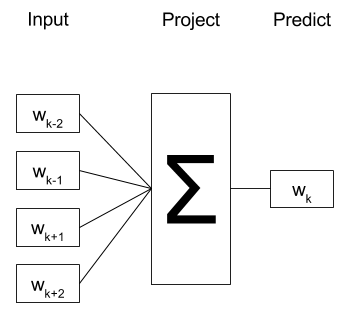
\includegraphics[width=\linewidth,left]{cbow.png}
  }
  \centering\tcbox[nobeforeafter,minipage,width=0.45\linewidth]{
    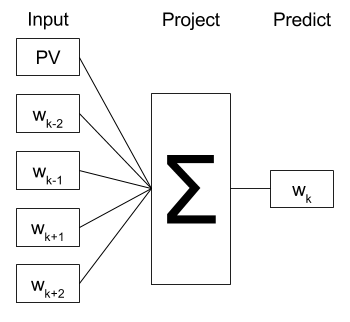
\includegraphics[width=\linewidth,right]{pbow.png}
  }
  \caption{Graphical representation of the ~\texttt{word2vec} (left)
           and ~\texttt{doc2vec} (right) algorithms.}
  \label{fig:cbow}
\end{figure}
Mikolov \etal show that these learnt word vectors not only retain semantic
information, but also relational information; for example, the result of
$\text{vec(king)} - \text{vec(man)} + \text{vec(woman)} \approx
\text{vec(queen)}$.

\subsection*{Paragraph Vectors}
In 2014, Le and Mikolov presented a method of altering the \texttt{word2vec}
algorithm to jointly train vector representations of documents in addition
to word vectors~\cite{le2014distributed}. This method is based on the idea of
basically adding a ``context vector", representing an individual document, to
each optimization. The process of learning these document vectors is equivalent
to that of learning word vectors in the \texttt{word2vec} algorithm, except an
additional paragraph vector (representing the document a given text sample comes
from) is added - see Figure~\ref{fig:cbow} for a graphical representation of the
difference. This modified \texttt{word2vec} algorithm is called
\texttt{doc2vec}.\\
Further exploration by Lau \etal shows that the \texttt{doc2vec} algorithm
provides many of the same interesting properties that \texttt{word2vec} can
provide~\cite{lau2016empirical}. Not only do the document vectors capture
semantic information, they \textit{also} capture relations: famous singers
are located in similar places, and using document vectors trained on wikipedia
pages, ``Lady Gaga" - ``America" + ``Japan" is closest to ``Ayumi Hamasaki",
a famous Japanese singer~\cite{dai2015document}.

\section*{Data Collection}

\subsection*{Data Sources}
We used three sources of data. Firstly, we use Maas' IMDB set~\cite{maas2011}
for verification and English language documents which can be found at
\url{http://ai.stanford.edu/~amaas/data/sentiment/}. Secondly, we used The
Wikimedia Foundation's English Wikipedia data dump~\cite{wikidatadump2016} as
a source for English language documents. We downloaded the full wiki dump from
\url{https://dumps.wikimedia.org/enwiki/20160820/}. Lastly, we used The
Chromium Project's Chromium repository~\cite{chromium2016} as a source for
source code documents. We cloned the repository at revision
\href{https://github.com/nwjs/chromium.src/commit/4fe31bb06cf458234d7017950a8b2b82427487c8}
{4fe31bb06cf458234d7017950a8b2b82427487c8}.

\subsection*{Data Scale}
The IMDB dataset contains a total of 100,000 files. Half are labelled as either a
positive or negative reviews, and the remainder are unlabelled. It is 346MB in size
and contains 23 million words, from a vocabulary of 90 thousand words.\\
The English Wikipedia Dataset is a single XML file, 13GB compressed and
55GB uncompressed. It contains 16 million pages, however this includes
redirects and meta-pages such as categories and portals, and therefore only
5 million of these are useful as documents. Excluding markup, this dataset contains
approximately 4 billion words.\\
The Chromium codebase is 2.6GB in size, and contains $245$ thousand files.
Of these, $23$ thousand are C and \CPP files, which contain $4.8$ million lines of
code and $608$ thousand lines of comments.

\subsection*{Data Format}
The fundamental requirements for the \texttt{doc2vec}~\cite{le2014distributed}
algorithm to work are that each document can be associated with the words in the
document, and that words in each document are just a series of words, i.e. no
excess punctuation or markup.\\
This requirement can easily be met by storing our set of documents as a newline
separated list of space separated tokens. The following example shows how a
simple document set might be transformed into this file format:\\
$$ \{\text{``My cow was sick, but now it is better."},
    \text{``Apples are nice.",
    \text{``Amazing results!"}}\} $$\\
Convert all text to lowercase and remove all punctuation:\\
$$ \{\text{``my cow was sick but now it is better"},
    \text{``apples are nice",
    \text{``amazing results"}}\} $$\\
Concatenate documents, separated by newlines:\\
\begin{align*}&\texttt{my cow was sick but now it is better}\\
&\texttt{apples are nice}\\
&\texttt{amazing results}\\\end{align*}
This format is simple to produce, simple to parse, and - given that the
\texttt{doc2vec} algorithm needs to process every word anyway - is efficient
to read. Perhaps more importantly, especially for large datasets like the
Chromium dataset, this storage format has no storage requirements in excess
of just the raw text in the files.

\subsection*{Data Processing}
To transform the data into the format previously described, some data processing
is required. All programs that we used to transform the datasets are available at
\url{https://github.com/mbd-doc2vec-team/mbd-doc2vec/tree/master/data-processing}.

\subsubsection*{IMDB Dataset}
The IMDB dataset needed minimal processing. The bulk of the work had already been
performed by the authors of the dataset. Beyond what had already been done,
punctuation, symbols and elements of markup were removed, and each document
concatenated into a file as discussed in the previous section.

\subsubsection*{Wikipedia Dataset}
The Wikipedia dataset required extensive pre-processing, with each document
needing to be parsed from the XML, and the plain text extracted from the wiki
markup. Additionally, ``fake" documents (e.g. portals, category pages) were
removed. Each wiki page was then tokenized and stored in a file as previously
stated.

\subsubsection*{Chromium Dataset}
The Chromium codebase required extensive pre-processing as well, with each \CPP
file being tokenized and having unicode characters (e.g. ¿) removed.
Unlike the other two datasets, because punctuation and uppercase/lowercase
distinctions are semantically significant in code, we retained punctuation and
the original casing in tokens.
Each comment and string literal was then tokenized as well, with punctuation
being removed from these tokens only, and the resulting tokens being stored as
discussed in the previous section. For an example of this process, the
document
\begin{align*}
&\texttt{// Frobulates the bar, in an efficient manner.}\\
&\texttt{void Frobulate(Bar \&bar);}\\
\end{align*}
would be represented by a line in the file as follows\\
\begin{align*}
\texttt{Frobulates the bar in an efficient manner void Frobulate ( Bar \& bar ) ;}
\end{align*}


\section*{Experiments}
Following are details as to how we carried out our experiments.
Full source code to do this can be found at
\url{https://github.com/mbd-doc2vec-team/mbd-doc2vec}, and full datasets
can be obtained as listed in the ``Data Sources" section of this paper.

\subsection*{IMDB Dataset}
The experimentation was undertaken with the method as follows.

\renewcommand\labelitemi{{\boldmath$\cdot$}}
\begin{description}
  \item Preprocessing
    \begin{itemize}
      \item The entire set of 100,000 documents were processed as described
            in the previous sections.
            The reason for concatenating all documents into a single file
            is that the dataset is small and can comfortably fit within memory,
            so it does not suffer from this simplification.
    \end{itemize}
  \item Training
    \begin{itemize}
      \item One of the co-authors of the original paper, Mikolov, provided
            some guidance and recommended the use of gensim's skip-gram model,
            which is trained for 20 iterations on the entire corpus of reviews.
      \item After each iteration, the order of the documents is randomized.
    \end{itemize}
  \item Evaluation
    \begin{itemize}
      \item The training document vectors are paired with their labels and
            a logistic regression is calculated to fit the training data.
      \item Prediction of sentiment using the testing document vectors takes
            place and the accuracy of the prediction versus the actual labels
            is reported.
    \end{itemize}
\end{description}

\subsection*{Wikipedia Dataset}

\subsection*{Chromium Dataset}


\section*{Results}

\subsection*{IMDB Dataset}
Through experimentation and switching from a neural network
based approach to a logistic regression, the final best accuracy
achieved whilst attempting to replicate the results was 89.4\%.\\
Being unable to replicate the results of Le and Mikolov in
\cite{le2014distributed}, some research into the result was
conducted. Many others were trying their hardest to replicate these
results, but ultimately the co-author Mikolov, who was not involved
in the experimentation found the issue.\\
This was reported in~\cite{mesnil2014ensemble}, where Mikolov
states the 92.6\% accuracy is achievable using hierarchical softmax
``only when the training and test data are not shuffled. Thus, we
consider this result to be invalid''. We therefore confirm this
non-replication.

\subsection*{Wikipedia Dataset}

\subsection*{Chromium Dataset}


\section*{Conclusion}


\subsection*{Future Work}

\printbibliography

\end{document}
